
%\documentclass[mathserif]{beamer}
\documentclass[10pt]{beamer}
%\usetheme{Goettingen}
%\usetheme{Warsaw}
\usetheme[progressbar=frametitle]{metropolis}



% \usepackage[english, activeacute]{babel}
% \usepackage[utf8]{inputenc}
% \usepackage{amsmath, amssymb}
% \usepackage{dsfont}
% \usepackage{graphics}
% \usepackage{cases}
% \usepackage{graphicx}
% \usepackage{pgf}
% \usepackage{epsfig}
% \usepackage{amssymb}
% \usepackage{multirow}	
% \usepackage{amstext}
% \usepackage[ruled,vlined,lined]{algorithm2e}
% \usepackage{amsmath}
% \usepackage{epic}
% \usepackage{epsfig}
% \usepackage{fontenc}
% \usepackage{framed,color}
% \usepackage{palatino, url, multicol}
% \usepackage{emoji}
% \usepackage{booktabs}
% \usepackage[scale=2]{ccicons}
% \usepackage[defaultsans]{FiraSans}

\usepackage{appendixnumberbeamer}

\usepackage{booktabs}
\usepackage[scale=2]{ccicons}

\usepackage{pgfplots}
\usepgfplotslibrary{dateplot}

\usepackage{xspace}
\newcommand{\themename}{\textbf{\textsc{metropolis}}\xspace}
\usepackage{emoji}

%\algsetup{indent=2em}
\newcommand{\factorial}{\ensuremath{\mbox{\sc Factorial}}}
\newcommand{\BIGOP}[1]{\mathop{\mathchoice%
{\raise-0.22em\hbox{\huge $#1$}}%
{\raise-0.05em\hbox{\Large $#1$}}{\hbox{\large $#1$}}{#1}}}
\newcommand{\bigtimes}{\BIGOP{\times}}
\vspace{-0.5cm}
\title{Natural Language Processing \\ 01. Introduction}
\vspace{-0.5cm}
\author[Juan José Alegría]{Juan José Alegría} 
\setbeamerfont{footnote}{size=\tiny}
 

\date{March 11, 2025}

\begin{document}
\begin{frame}
\titlepage


\end{frame}


\begin{frame}{Disclaimer}

\begin{itemize}
    \item These slides are \textbf{heavily} based on Felipe Bravo's work
    \item At the same time, a significant part of the content presented in his slides took inspiration from other resources such as textbooks and publications.  
    \begin{itemize}
    
    
        \item  The neural network part of the course is based on Yoav Goldberg's book \cite{goldberg2017neural}
        \item Non-neural network topics, such as probabilistic language models, are taken from Michael Collins' Columbia course \cite{collins2013language}.
        \item Also from the draft of the third edition of Dan Jurafsky and James H. Martin's book \cite{JurafskyBook}.
        \item In addition, some slides have been adapted from online tutorials and other courses, such as Christopher Manning's Stanford course\footnote{\url{ttp://web.stanford.edu/class/cs224n/}}. 
    \end{itemize}
\end{itemize}

\end{frame}

\begin{frame}{Table of contents}
  \setbeamertemplate{section in toc}[sections numbered]
  \tableofcontents%[hideallsubsections]
\end{frame}

\section{What is Natural Language Processing?}

\begin{frame}{What is Natural Language Processing?}
\begin{quote}
    ``Natural language processing (NLP) is the field of designing methods and algorithms that take as input or produce as output unstructured, natural language data.'' \\ \cite{goldberg2017neural}
\end{quote}
\end{frame}


\begin{frame}{Why do we need/want Natural Language Processing?}
\begin{itemize}


\item The amount of digitized textual data generated daily is huge (e.g., the Web, social media, medical records, digitized books) \to \> there is information there that we may want to retrieve!

\item We would like to do many things that involve text \to \> translation, summarization, question answering, etc.

\item Tasks \emoji{eyes}

\end{itemize}
\end{frame}


\begin{frame}{Natural Language Processing}

    \begin{figure}[h]
        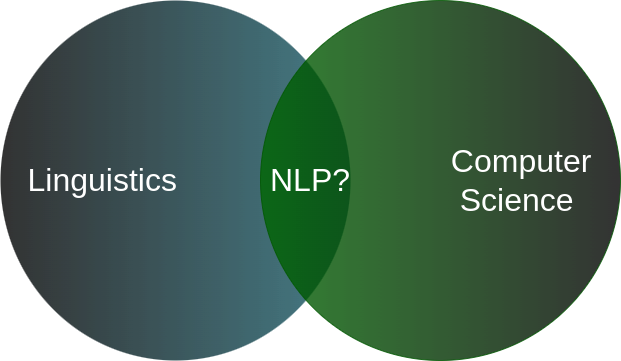
\includegraphics[scale = 0.4]{pics/nlp_intersection.png}
    \end{figure}

    
    \texttt{Important:} There are two related fields at the intersection of linguistics and computer science: Natural Language Processing and Computational Linguistics

\end{frame}

\begin{frame}{Natural Language Processing and Computational Linguistics}

\begin{itemize}
\item Natural language processing (NLP) develops methods for solving practical problems involving language \cite{JohnsonMLSS}. \\

\begin{itemize}
\item Automatic speech recognition.
\item Machine translation.
\item Information retrieval from documents.
\end{itemize}

\item Computational linguistics (CL) studies the computational processes underlying (human) language.

\begin{itemize}
 \item How do we understand language?
 \item How do we produce language?
 \item How do we learn language?
\end{itemize}

\item Similar methods and models are used in NLP and CL, but with a different focus. In CL, language is the object of study.
\end{itemize}

\end{frame}

\section{Language}

\begin{frame}{Language can be difficult}


    \begin{figure}[h]
        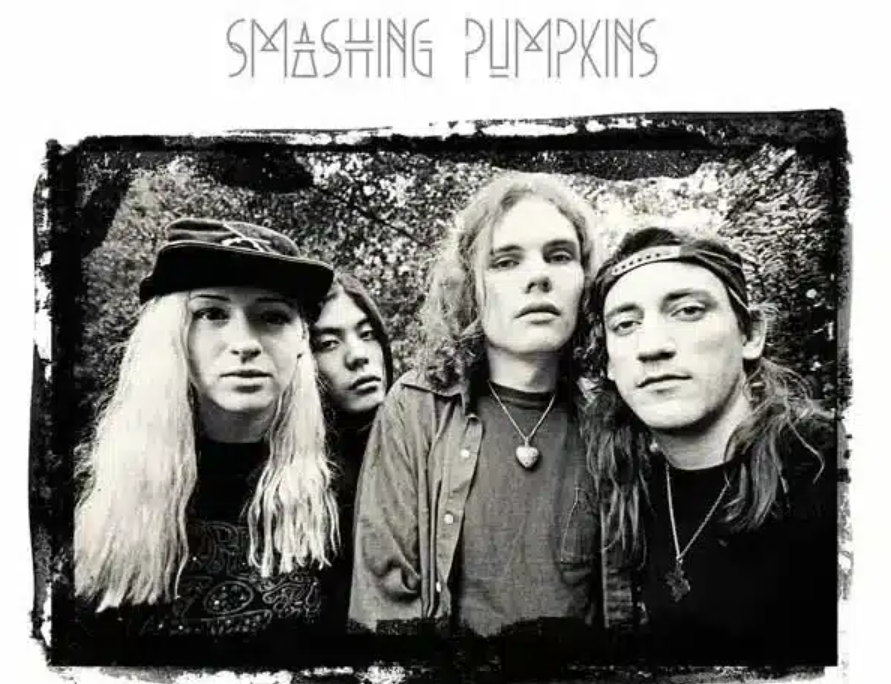
\includegraphics[scale = 0.4]{pics/smashing1.png}
    \end{figure}
    

\end{frame}


\begin{frame}{Language can be difficult}


    \begin{figure}[h]
        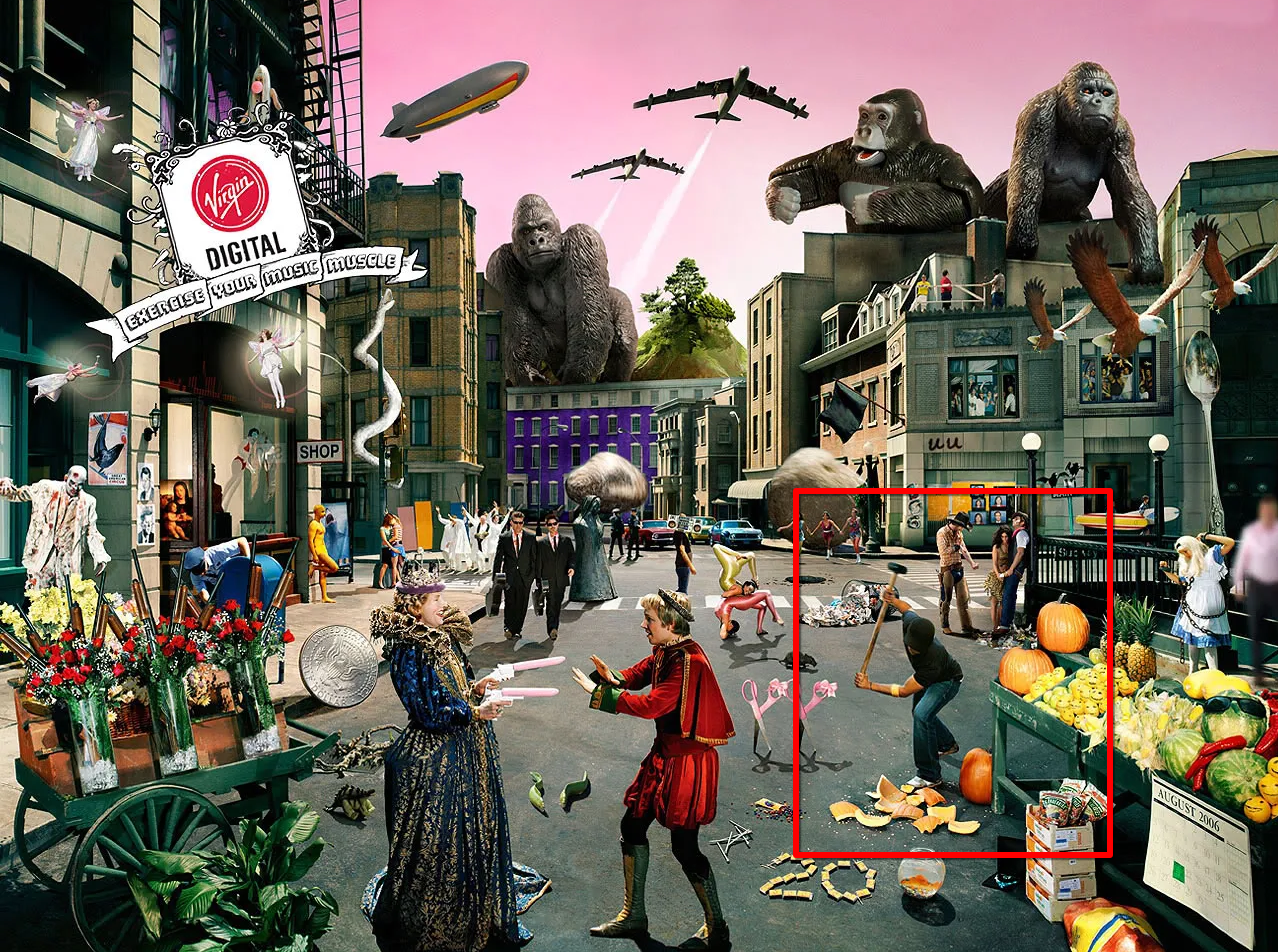
\includegraphics[scale = 0.3]{pics/smashing2.png}
    \end{figure}
    

\end{frame}


\begin{frame}{5 Challenging Properties of Human Language}

\begin{enumerate}        
\item \textbf{Ambiguity}: Human language is highly ambiguous.
\begin{itemize}
 \item For example: \emph{I ate pizza with friends} vs. \emph{I ate pizza with olives} vs. \emph{I ate pizza with a fork}.
\item All these sentences have similar grammatical properties but differ radically in what the prepositional phrase modifies: (1) the pronoun ``I'', (2) the noun ``pizza'', (3) the verb ``eat''. 
\end{itemize}
\item \textbf{Dynamism}: Language is ever changing and evolving (e.g, Hashtags in Twitter).
\end{enumerate}


\end{frame}

\begin{frame}{5 Challenging Properties of Human Language}

\begin{enumerate}  
\setcounter{enumi}{2}
\item \textbf{Discreteness}: we cannot infer the relation between two words from the letters they are made of (e.g., hamburger and pizza). 
\item \textbf{Compositionality}: the meaning of a sentence goes beyond the individual meaning of their words. 
\item \textbf{Sparseness}: The way in which words
(discrete symbols) can be combined to form meanings is practically infinite.
\end{enumerate}

\end{frame}

\section{NLP and Machine Learning}

\begin{frame}{Natural Language Processing and Machine Learning}
\begin{itemize}

\item Although we humans are great users of language, we are also very poor at formally understanding and describing the rules that govern language.

\item Understanding and producing language using computers is highly challenging.
\item The best known set of methods for dealing with language data is based on supervised machine learning.
\item Supervised machine learning: attempt to infer usage patterns and regularities from a set of pre-annotated input and output pairs (a.k.a training dataset).

\end{itemize}
\end{frame}

\begin{frame}{Example: Sentiment classification}
\begin{itemize}
    \item Objective: Classify tweets as positive or negative
    \item We already have a \textbf{corpus} of labeled tweets (positive/negative)
    \item How can we train a classifier?
\end{itemize}

\begin{figure}[h]
    \includegraphics[scale = 0.3]{pics/tweets.png}
\end{figure}

\end{frame}

\begin{frame}{Input: Bag of Words}

\begin{figure}[h]
    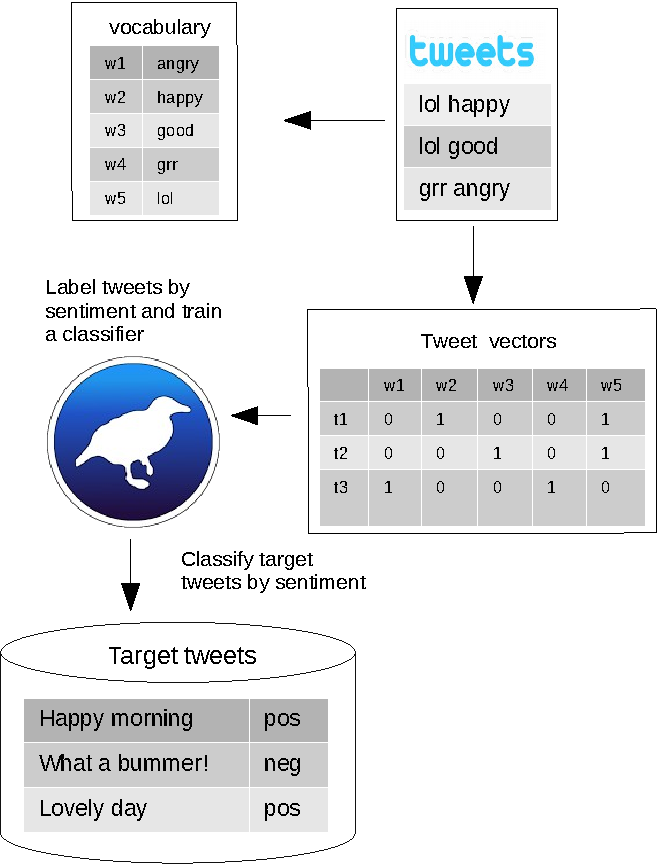
\includegraphics[scale = 0.5]{pics/bagOfwordsClassification.pdf}
\end{figure}

\end{frame}

\begin{frame}{Supervised Learning: Support Vector Machines (SVMs)}
\begin{itemize}

\item Idea: Find a hyperplane that separates the classes with the maximum margin (largest separation). 

\begin{figure}[h]
    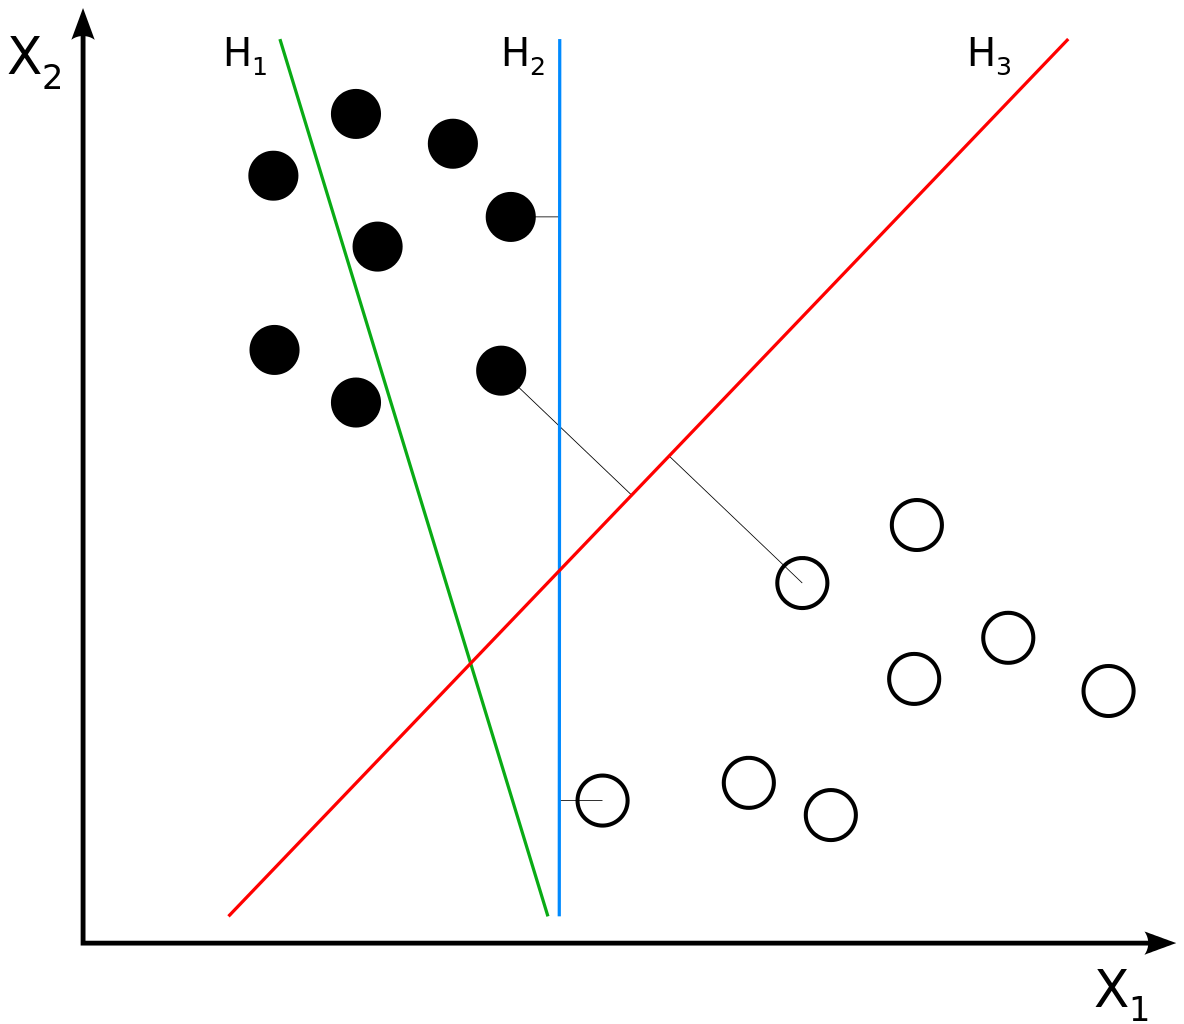
\includegraphics[scale = 0.15]{pics/SVM.png}
\end{figure}

\item   
$H_3$ separates the classes with the maximum margin. 

\end{itemize}

\footnotetext[2]{Image source: \href{https://en.wikipedia.org/wiki/Support_vector_machine}{\textit{Wikipedia} - Support vector machine}}


\end{frame}

\begin{frame}{Supervised Learning: Random Forest}
\begin{itemize}

\item Idea: Train several (almost) independent trees and then perform majority voting

\begin{figure}[h]
    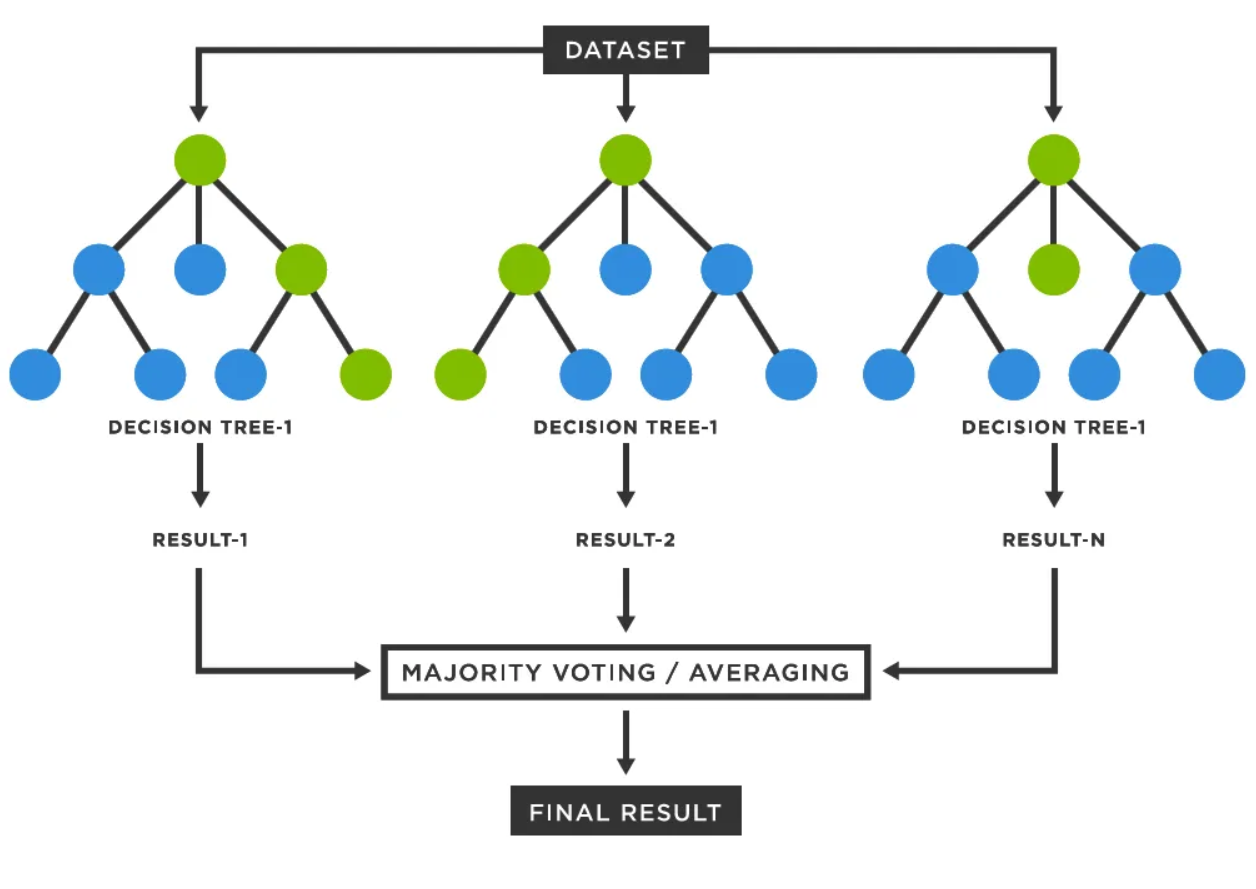
\includegraphics[scale = 0.3]{pics/random_forest.png}
\end{figure}

\end{itemize}

\footnotetext[3]{Image source: \href{https://medium.com/@denizgunay/random-forest-af5bde5d7e1e}{\textit{Medium} - Random Forests}}


\end{frame}


\begin{frame}{Supervised Learning: (shallow) Neural Network}
\begin{itemize}

\item Idea: Train a neural network (a.k.a. multilayer perception), using the bag of words as input

\begin{figure}[h]
    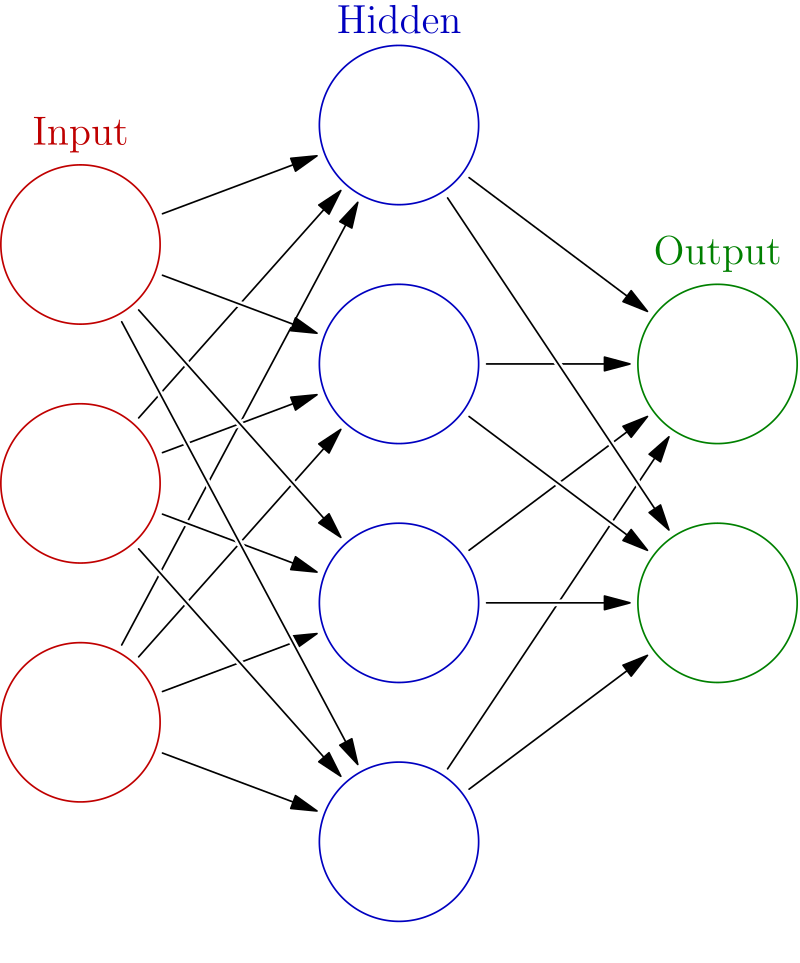
\includegraphics[scale = 0.2]{pics/neural_network.png}
\end{figure}

\end{itemize}

\footnotetext[4]{Image source: \href{https://en.wikipedia.org/wiki/Neural_network_\%28machine_learning\%29}{\textit{Wikipedia} - Neural network (machine learning)}}
\end{frame}


\begin{frame}{Supervised Learning: Can we do better?}
\begin{itemize}

\item We can use several ML models, some that we don't even mentioned (KNN, naive bayes, etc)

\item But can we improve the input?

\item Maybe we can new features, not just counting words. 

\item This are called \textit{hand-crafted} features

\item Ideas?
\end{itemize}
\end{frame}

\begin{frame}{Hand-crafted features}
\begin{itemize}
\item Some hand-crafted features devised by the team that achieved the best performance \cite{Mohammad2013} in the ``Sentiment Analysis in Twitter task'' in the Semantic Evaluation Workshop (2013) \cite{Semeval2013}:
\begin{enumerate}

\item Word $n$-grams.
\item Character $n$-grams. 
\item Part-of-speech tags.

\item The number of elongated words (words with one character repeated more than two times).
\item The number of words with all characters in uppercase.
\item The presence of positive or negative emoticons.
\item The number of individual negations.
\item The number of contiguous sequences of dots, question marks and exclamation marks.
\item Features derived from polarity lexicons \cite{Mohammad2013}. 
\item Etc.
\end{enumerate}
\end{itemize}
\end{frame}

\begin{frame}{Hand-crafted features}
\begin{itemize}
\item Designing hand-crafted features is hard. Feature engineering requires domain knowledge and is usually a bottleneck in the process.
\item It would be nice if the models themselves were able to find the best way to represent the input \emoji{eyes} \emoji{eyes} \emoji{eyes}
\end{itemize}
\end{frame}


\begin{frame}{Deep Learning}
    \begin{figure}[h]
        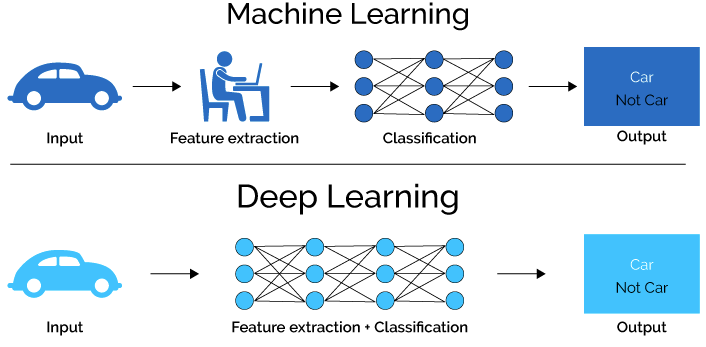
\includegraphics[scale = 0.25]{pics/MLvsDL.png}
    \end{figure} 
    \begin{itemize}
        \item In Deep Learning, we give the input to the model with ``little'' preprocessing: the model itself learns how to best represent the input.
        \item Deep Learning yields state-of-the-art results in most NLP tasks. 
        \item Large amounts of training data and faster multicore GPU machines are key in the success of deep learning. 
        \item \textbf{Neural networks} and \textbf{word embeddings} play a key role in modern NLP models.
    \end{itemize}
\end{frame}

\section{NLP Tasks}

\begin{frame}{Tasks}
\begin{itemize}
    \item There are many possible problems that we would like to tackle using NLP methods; these are usually called \textbf{\textit{tasks}}.

    \item Some examples:
    \begin{itemize}
        \item \textbf{Text classification}: given a document, classify it into one of several classes. E.g., classify a news article into \textit{SPORTS}, \textit{GOSSIP}, \textit{POLITICS} o \textit{ECONOMY}.
        \item \textbf{Sentiment Analysis}: classify a document according to its polarity. It's a type of text classification but with some particular nuances (sarcasm, irony, negations, etc)
        \item \textbf{Named Entity Recognition (NER)}: given a text, recognize and classify entities (people, places, organizations, etc). 
        \item \textbf{Parts-Of-Speech (POS) Tagging}: classify each word in the text into nouns, verbs, adjectives, etc.
        \item \textbf{Machine translation}: translate a sentence from a source language to a target language.
        \item \textbf{Question Answering}: given a paragraph $p$ and a question $q$, find in the $p$ the answer to $q$.
        \item Etc.
    \end{itemize}
\end{itemize}
    
\end{frame}

\begin{frame}{Tasks and data labeling}
\begin{itemize}
    \item We are in the supervised learning framework, so to train a model for any task, we need labeled data.
    \item Clearly, the labeling for each task is different.
    
    
\end{itemize}
\end{frame}

\begin{frame}{Data labeling for text classification}
\begin{figure}[h]
    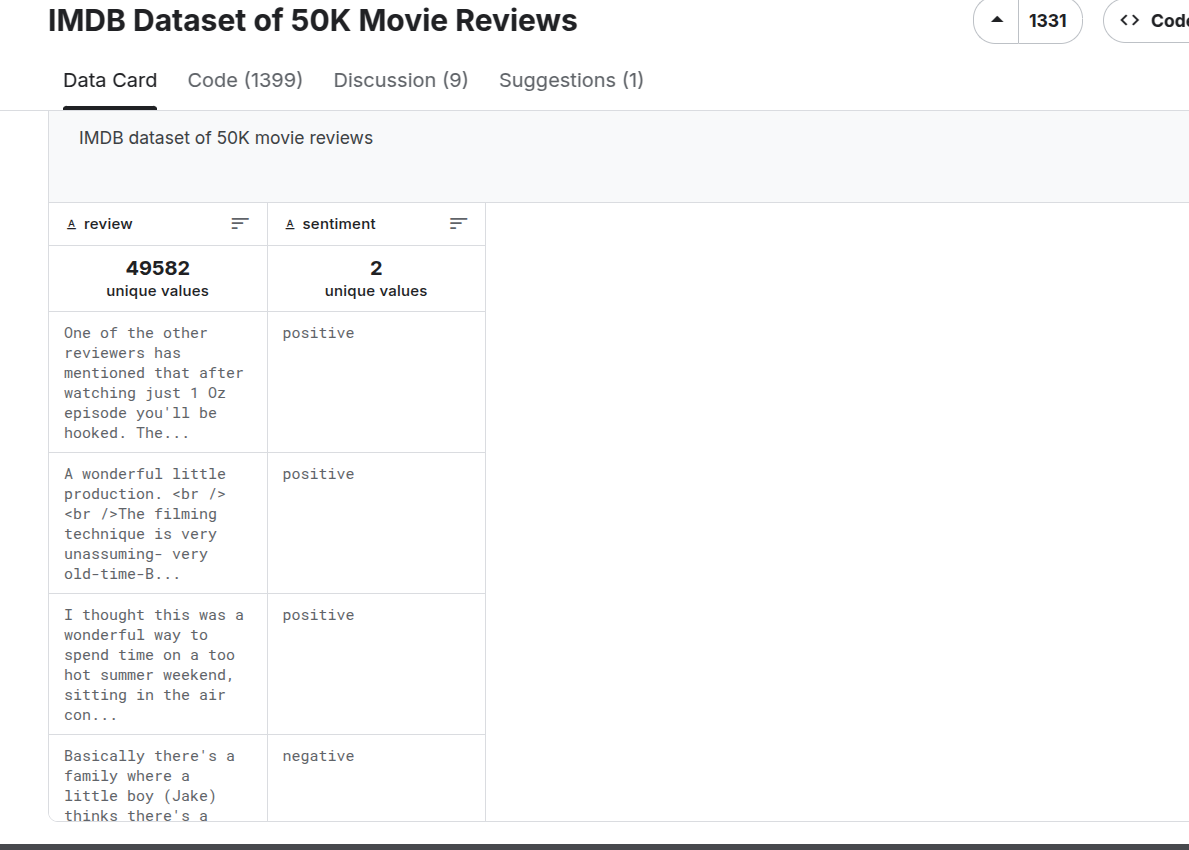
\includegraphics[scale = 0.32]{pics/label_classification.png}
\end{figure}

\footnotetext[5]{Source: \href{https://www.kaggle.com/datasets/lakshmi25npathi/imdb-dataset-of-50k-movie-reviews}{\textit{Kaggle} - IMDB Dataset of 50K Movie Reviews}}
\end{frame}

\begin{frame}{Data labeling for POS tagging and NER}
\begin{figure}[h]
    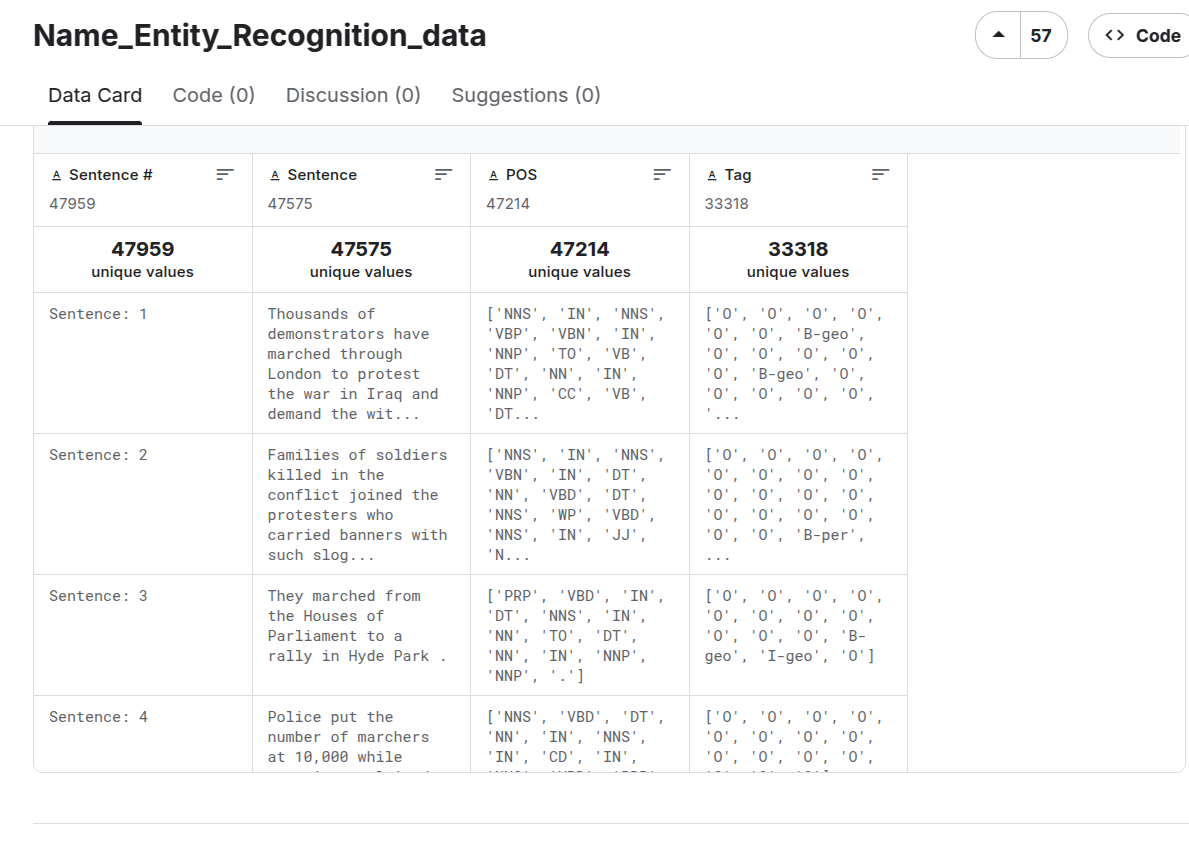
\includegraphics[scale = 0.32]{pics/label_pos_ner.png}
\end{figure}

\footnotetext[6]{Source: \href{https://www.kaggle.com/datasets/vimlendusharma/name-entity-recognition-data}{\textit{Kaggle} - Name\_Entity\_Recognition\_data}}
\end{frame}

\begin{frame}{Data labeling for machine translation}
\begin{figure}[h]
    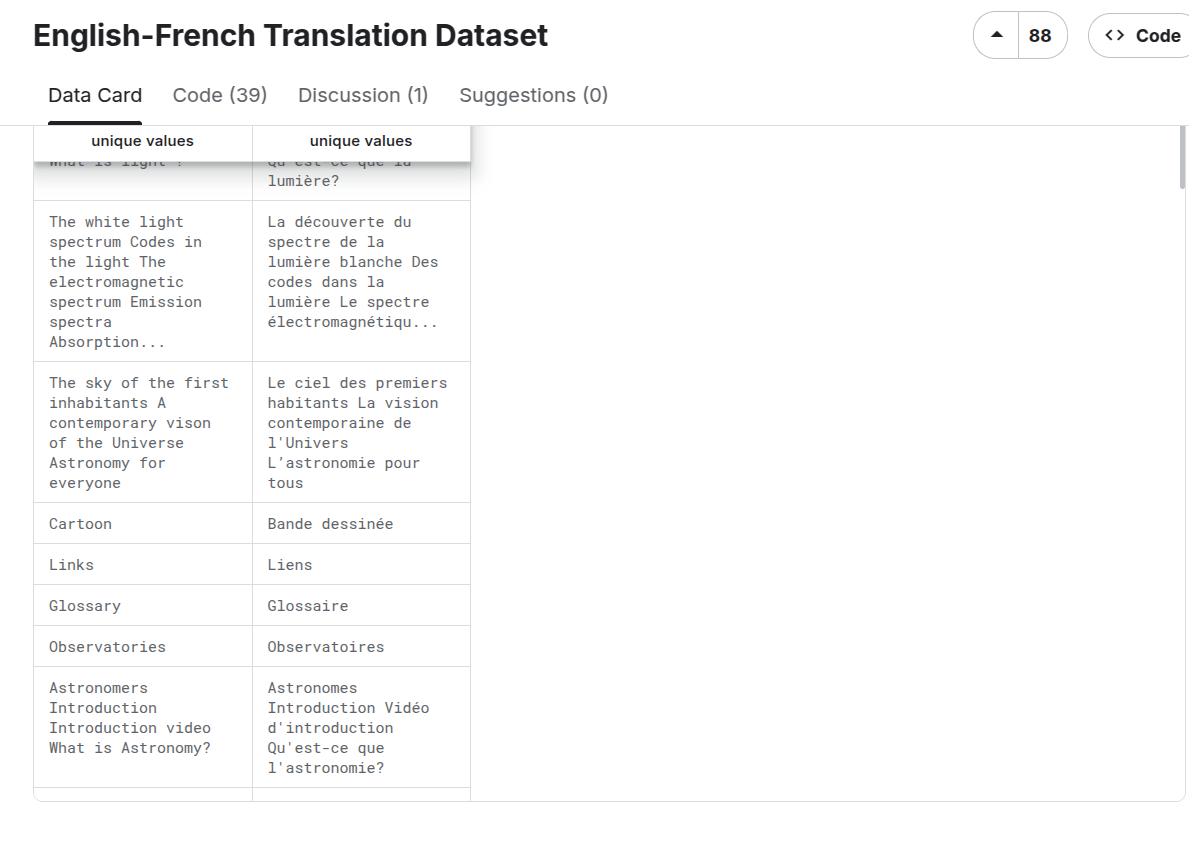
\includegraphics[scale = 0.32]{pics/label_translation.png}
\end{figure}

\footnotetext[7]{Source: \href{https://www.kaggle.com/datasets/dhruvildave/en-fr-translation-dataset}{\textit{Kaggle} - English-French Translation Dataset}}
\end{frame}


\section{Brief history of NLP}

\begin{frame}{NLP History}
NLP progress can be divided into three main waves: 1) rationalism, 2) empiricism, and 3) deep learning \cite{deng2018deep}.
\begin{itemize}
\item \textbf{(1950 - 1990) Rationalism:} approaches endeavored to design hand-crafted rules to incorporate knowledge and reasoning mechanisms into intelligent NLP systems (e.g,  ELIZA for simulating a Rogerian psychotherapist, MARGIE for structuring real-world information into concept ontologies).
\item \textbf{(1991 - 2009) Empiricism:} characterized by the exploitation of data corpora and of (shallow) machine learning and statistical models (e.g., Naive Bayes, HMMs, IBM translation models).
\item \textbf{(2010 - ) Deep Learning:} feature engineering (considered as a bottleneck) is replaced with representation learning and/or deep neural networks (e.g., \href{https://www.deepl.com/translator}{DeepL Translator}). A very influential paper in this revolution: \cite{collobert2011natural}.
\end{itemize}

\end{frame}


\begin{frame}{A fourth wave?}

\begin{itemize}
\item Large Language Models (LLMs) like GPT, DeepSeek R1, Llama, Gemino, etc., are deep neural networks trained on large corpora (hundreds of billions of tokens) and a large parameter space (billions) to predict the next word from a fixed-size context.
\item One of the most striking features of these models is their ability for few-shot, one-shot, and zero-shot learning, often referred to as ``in-context learning''.
\item This implies their capacity to acquire new tasks with minimal human-annotated data, simply by providing the appropriate instruction or prompt.
\item Thus, despite being rooted in the deep learning paradigm, they introduce a disruptive approach to NLP.
\end{itemize}
\end{frame}

\section{Roadmap and evaluations}

\begin{frame}{Roadmap}
Unit 1: Foundations of NLP
\begin{enumerate}
    \item Introduction to NLP
    \item Vector Semantics
    \item Fundamental questions about language
    \item Probabilistic language models
    \item Linear models
\end{enumerate}
\end{frame}

\begin{frame}{Roadmap}
Unit 2: Neural networks
\begin{enumerate}
\setcounter{enumi}{4}
    \item Neural Networks
    \item Word Vectors
    \item Recurrent Neural Networks
    \item Sequence-to-sequence + Attention
    \item Transformers + BERT
\end{enumerate}
\end{frame}

\begin{frame}{Roadmap}
Unit 3: Large Language Models and applications
\begin{enumerate}
\setcounter{enumi}{9}
    \item GPT + LLMs and emergent abilities
    \item Retrieval Augmented Generation
    \item Interpretability
    \item Agents
    \item Ethics
\end{enumerate}
\end{frame}

\begin{frame}{Evaluations}
\begin{itemize}
    \item NC: 2 tests (``controles''): after Unit 1 and Unit 2
    \item NP: 1 group presentation of a paper (selected by you from a set of options we'll provide) the last week of the semester
    \item NT: 3 group homework assignment (``tareas grupales'')
\end{itemize}
Final grade: (NC + NP + NT) / 3
\end{frame}

\begin{frame}{Other stuff}
\begin{itemize}
    \item \textbf{Course repository}: \url{https://github.com/dccuchile/CC6205}
    \item The schedule will be listed there!
\end{itemize}    
\end{frame}

\begin{frame}[allowframebreaks]\scriptsize
\frametitle{References}
\bibliography{bio}
\bibliographystyle{apalike}
%\bibliographystyle{flexbib}
\end{frame}  
%%%%%%%%%%%%%%%%%%%%%%%%%%%

\end{document}
